\subsection{3.1配分函数和分布函数}
我们的第一项任务是讨论理想链模型的配分函数和分布函数是如何在外场存在的情况下进行修改的。我们从离散高斯链开始。
\subsubsection{3.1.1离散高斯链}
主要感兴趣的外场是一个空间变化的化学势场$w(\mathrm{r})$,它作用于离散高斯链的$N+1$个珠子上,我们再次采用图2.1和2.3节的表示法。势能可以写成
\begin{equation}
\begin{aligned}
U(\mathrm{r}^{N+1})&=U_0(\mathrm{r}^{N+1})+U_1(\mathrm{r}^{N+1})\\
&=\sum\limits_{i=1}^Nh(\left|\mathrm{r}_i-\mathrm{r}_{i-1}\right|)+k_BT\sum\limits_{i=0}^Nw(\mathrm{r}_i)
\end{aligned}
\end{equation}
这里$h(x)=3k_BTx^2/(2b^2)$和$\mathrm{r}^{N+1}$是$N+1$个珠子坐标$(\mathrm{r}_0,\mathrm{r}_1,\cdots,\mathrm{r}_N)$的缩写。$N$键上的第一个和是$U_0$,这是离散高斯链的调和伸缩能(harmonic stretching energy)。$N+1$微球上的第二个和计算了每个珠子与势场$k_BTw(\mathrm{r})$的相互作用能。另一种表示外部势能项$U_1(\mathrm{r}^{N+1})$的方法是
\begin{equation}
\beta U_1(\mathrm{r}^{N+1})=\int\mathrm{d}\mathrm{r}w(\mathrm{r})\hat{\rho}(\mathrm{r})
\end{equation}
其中段的微观密度由下式定义:
\begin{equation}
\hat{\rho}(\mathrm{r})=\sum\limits_{i=0}^N\delta(\mathrm{r}-\mathrm{r}_i)
\end{equation}
这种微观密度显然是$\mathrm{r}$的非常奇异的函数,并且显然地依赖于珠子坐标$\mathrm{r}^{N+1}$。方程(3.2)表示的事实是,势场$w(\mathrm{r})$可以看作是一个空间变化的化学势场,它是热力学共轭于段密度的化学势场(Chandler,1987)。

特别令人感兴趣的是,受外部势场$w(\mathrm{r})$,$Z[w]$作用的链的配分函数与理想链的配分函数$Z_0$的比率。
\begin{equation}
Q(w)\equiv\frac{Z[w]}{Z_0}=\frac{\int\mathrm{d}\mathrm{r}^{N+1}\exp[-\beta U(\mathrm{r}^{N+1})]}{V(\int\mathrm{d}\mathbf{b}\exp[-\beta h(\left|\mathbf{b}\right|)])^N}
\end{equation}
在该表达式的分母中,使用了(2.27)式,它将$Z_0$表示为键向量上的体积$V$乘以$N$个独立(体积)积分,如符号所示,归一化配分函数$Q[w]$可以看作是外部势场$w(r)$的函数。

下一步是将等式(3.4)的分母中的$\int\mathrm{d}\mathbf{b}\exp[-\beta h(\left|\mathbf{b}\right|)]$的$N$个因子与分子中的$\exp[-\beta h(\left|\mathrm{r}_i-\mathrm{r}_{i-1}\right|)]$的$N$个因子相关联。回顾离散高斯链的归一化键转移概率的定义,方程(2.34)
\begin{equation}
\Phi(\mathrm{r})=\frac{\exp[-\beta h(\left|\mathrm{r}\right|)]}{\int\mathrm{d}\mathrm{r}\exp[-\beta h(\left|\mathrm{r}\right|)]}=\left(\frac{3}{2\pi b^2}\right)^{3/2}\exp\left(-\frac{3\left|\mathrm{r}\right|^2}{2b^2}\right)
\end{equation}
使等式(3.4)重写为
\begin{equation}
\begin{aligned}
Q[w]=\frac{1}{V}\int\mathrm{d}\mathrm{r}^{N+1}&[e^{-w(\mathrm{r}_N)}\Phi(\mathrm{r}_N-\mathrm{r}_{N-1})e^{-w(\mathrm{r}_{N-1})}\Phi(\mathrm{r}_{N-1}-\mathrm{r}_{N-2})\\
&\cdots e^{-w(\mathrm{r}_2)}\Phi(\mathrm{r}_2-\mathrm{r}_1)e^{-w(\mathrm{r}_1)}\Phi(\mathrm{r}_1-\mathrm{r}_0)e^{-w(\mathrm{r}_0)}]
\end{aligned}
\end{equation}
这个表达式可以按以下方式递归构建。我们对整数$j$定义了一个泛函$q(\mathrm{r},j;[w])$通过
\begin{equation}
q(\mathrm{r},0;[w])=\exp[-w(\mathrm{r})]
\end{equation}
和对$j=0,1,2,\cdots,N-1$
\begin{equation}
q(\mathrm{r},j+1;[w])=\exp[-w(\mathrm{r})]\int\mathrm{d}\mathrm{r}'\Phi(\mathrm{r}-\mathrm{r}')q(\mathrm{r}',j;[w]))
\end{equation}
因此,归一化的配分函数可以表示为
\begin{equation}
Q[w]=\frac{1}{V}\int\mathrm{d}\mathrm{r}q(\mathrm{r},N;[w])
\end{equation}
在上文中,$q(\mathrm{r},j;[w])$表示$j+1$个珠子链在$r$位置处的统计权重。该对象通常被称为链传播子,是外部势场$w(\mathrm{r})$的函数。方程(3.8)可以看作是一个Chapman-Kolmogorov方程,对于无场情况下概率密度$p_0(\mathrm{r},j)$,它与方程(2.33)严格类似。实际上,除了函数$p_0(\mathrm{r},j)$和$q(\mathrm{r},j;[w])$的不同归一化之外,方程(3.8)对于$w(\mathrm{r})\rightarrow 0$被看作是方程(2.33)。

需要注意的是,对于任何弹簧势$h(x)$,式子(3.7)-(3.9)都是成立的,条件是用适当的形式代替高斯模型式子(3.5)的跃迁概率密度$\Phi(\mathrm{r})$。参见式子(2.40),式子(3.7)-(3.9)适用于式子(2.41)等非线性珠弹簧模型。
\begin{figure}[H]
\centering
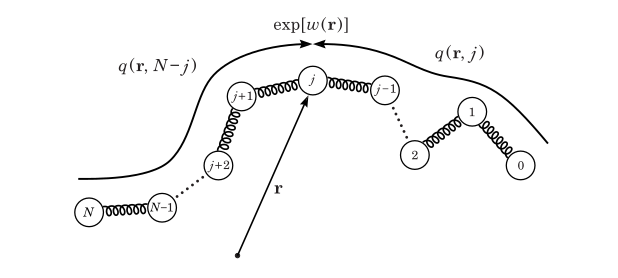
\includegraphics[scale=0.7]{./figures/Figure_1.png}
\end{figure}

































